\documentclass{beamer}

\usetheme{metropolis}
\usepackage{appendixnumberbeamer}


\usepackage[english]{babel}
\usepackage[sfdefault]{FiraSans}
\usepackage{amssymb,mathrsfs,mathtools}
\usepackage{amsfonts}
\usepackage{tikz,pgfopts,etoolbox,calc,ifxetex,ifluatex}
\usefonttheme[onlymath]{serif}

\setbeamercovered{highly dynamic}

\title{\textsc{A Bayesian model for data flow: BikeMi}}
\subtitle{}
\author{Andrea De Gobbis, Lorenzo Ghilotti, Giorgio Meretti}
\institute{Politecnico di Milano}
\logo{\includegraphics[width=15mm]{Politecnico_di_Milano}}
\date{November 22, 2019}
\usetheme{Goettingen}
\usecolortheme{dolphin}

\begin{document}
	\begin{frame}
	\maketitle	
\end{frame}


\begin{frame}{\textsc{Bike Sharing}}

\begin{columns}[c]
	\hspace{10pt}
	\begin{column}{0.5\textwidth}
		We aim to develop a Bayesian model for the analysis of the \alert{flow counts} on a \alert{complex network}.
	\end{column}
	\hspace{5pt}
	\vrule{}
	\hspace{10pt}
	\begin{column}{0.50\textwidth}
		 Application to the bike sharing platform \alert{BikeMi},\\ in Milan.
	\end{column}
\end{columns}

\begin{figure}[H]
	\centering
	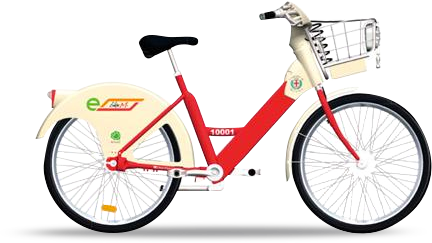
\includegraphics[width=0.6\linewidth]{pictures/bikemi.png} 
	\label{fig1}
\end{figure}
  
 
  
\end{frame}

\begin{frame}{\textsc{The Bike Sharing System}}
\begin{itemize}
	\item Bike sharing is a service in which bicycles are made available for \alert{shared use} to individuals on a short term basis for a price or free.
	\item BikeMi allows people to borrow a bike from a \alert{\textquotedblleft station\textquotedblright} and return it at another station belonging to the system.\\
	\ 
	\begin{figure}[H]
		\centering
		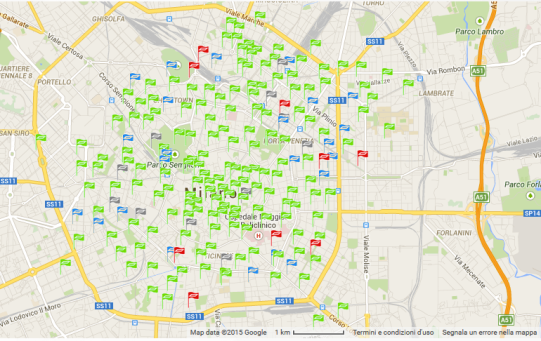
\includegraphics[width=0.7\linewidth]{pictures/mappa.png} 
		\label{fig2}
	\end{figure}
\end{itemize}
	
	
\end{frame}
	
\begin{frame}{\textsc{Dataset}}
	The data covers a period between 25/01/2016 and 07/03/2016, with a total of 35 thousand data points.
	\begin{itemize}[<+->]
		\item<1,2,3,4> Date;
		\item<2,3,4> Time of departure/arrival;
		\item<3,4> Station of departure/arrival;
		\item<4> Weekday: binary indicating if the day is in the weekend or not.
	\end{itemize}
\end{frame}

\begin{frame}{\textsc{Statistics on a Graph}}
	\onslide<1>
	{Setting $\implies$ \alert{complete directed graph} $\mathcal{G} = (V,E)$
	 
	 \begin{itemize}
	 	\item vertices $V$ representing the stations
	 	\item edges $E = \{(i,j)\}$: the weight of the edges will be the count flow of bikes.
	 \end{itemize} 
 	}
 
	\onslide<2>
	{
	As \alert{pre-processing} it was introduced a node clusterization using the \alert{DBSCAN} algorithm,\\ since many stations are very close to one another.
	}
\end{frame}

\begin{frame}{\textsc{A Basic Model for the Phenomenon}}
	The flow counts are modeled with a \alert{Poisson} distribution:
	
	\begin{equation}
	\begin{cases}
	
	Y_{ij} \sim \mathrm{Poi}(Y_{ij}|\mu_{ij}) \\
	\\
	
	\mu_{ij} = \mathrm{exp}\{\boldsymbol{\beta}\cdot \mathbf{x}_{ij}\}
	
	\end{cases}
	\end{equation}
	
	The means are derived through \alert{loglinear} regression.
	\begin{figure}[H]
		\centering
		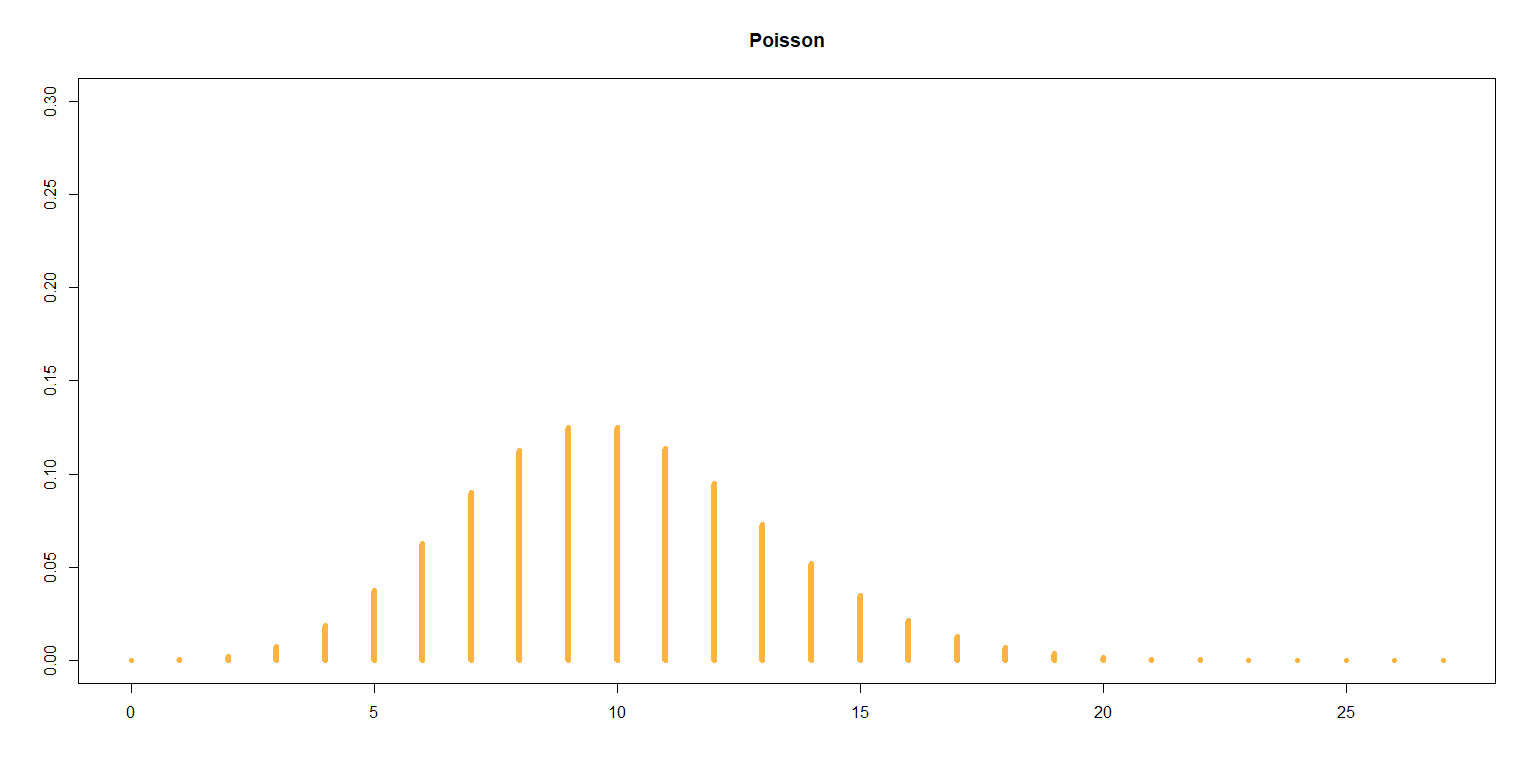
\includegraphics[width=0.75\linewidth]{pictures/mod1.png} 
		\label{fig1}
	\end{figure}
	
\end{frame}

\begin{frame}{\textsc{An Improved Model for the Phenomenon}}
We introduce a division in \alert{$K$ clusters}:

\begin{equation}
\begin{cases}

Y_{ij} \sim \mathrm{PM}(Y_{ij}|\boldsymbol{\mu}_{ij}, \boldsymbol{\lambda})
\\
\mathrm{PM}(\boldsymbol{\mu}_{ij}, \boldsymbol{\lambda}) = \sum_{k=1}^K \lambda_k\mathrm{Poi}(\mu_{ijk})
\\
\mu_{ijk} = \mathrm{exp}\{\boldsymbol{\beta}_k\cdot \mathbf{x}_{ij}\}
\end{cases}
\end{equation}

where $\lambda_k$ is the probability of belonging to group $k$.
\begin{figure}[H]
	\centering
	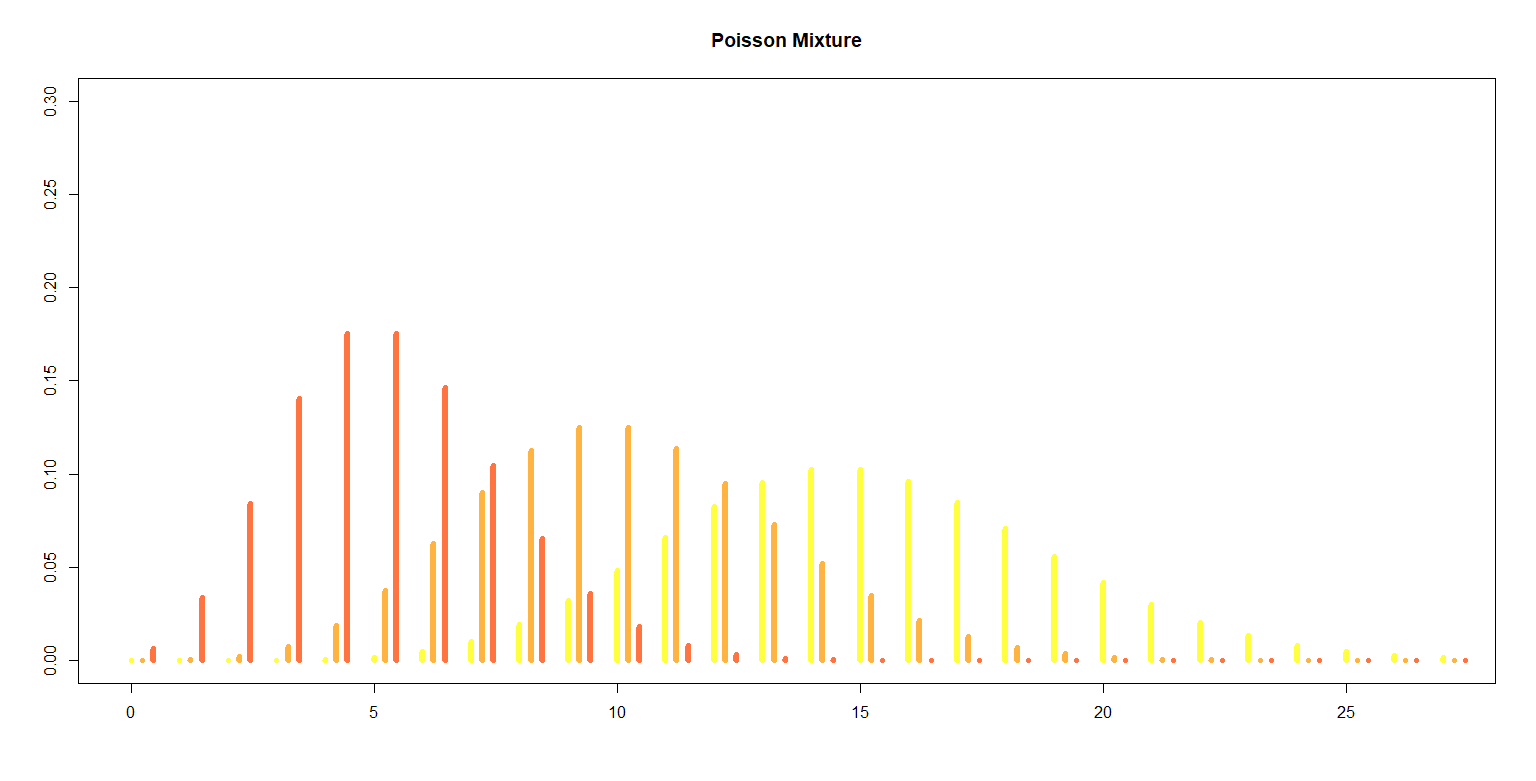
\includegraphics[width=0.75\linewidth]{pictures/mod2.png} 
	\label{fig1}
\end{figure}

\end{frame}

\begin{frame}{\textsc{A Proposed Model for the Phenomenon}}
	Since the model will determine the \alert{topology of the graph} we might desire a better \alert{control} on $\mathbb{P}(Y_{ij} = 0)$, they introduce a delta measure in $ 0 $.
	 $$Y_{ij} \sim \theta \delta_{0} + (1 - \theta)\mathrm{PM}(Y_{ij}|\boldsymbol{\mu}_{ij}, \boldsymbol{\lambda})$$
	 \begin{figure}[H]
	 	\centering
	 	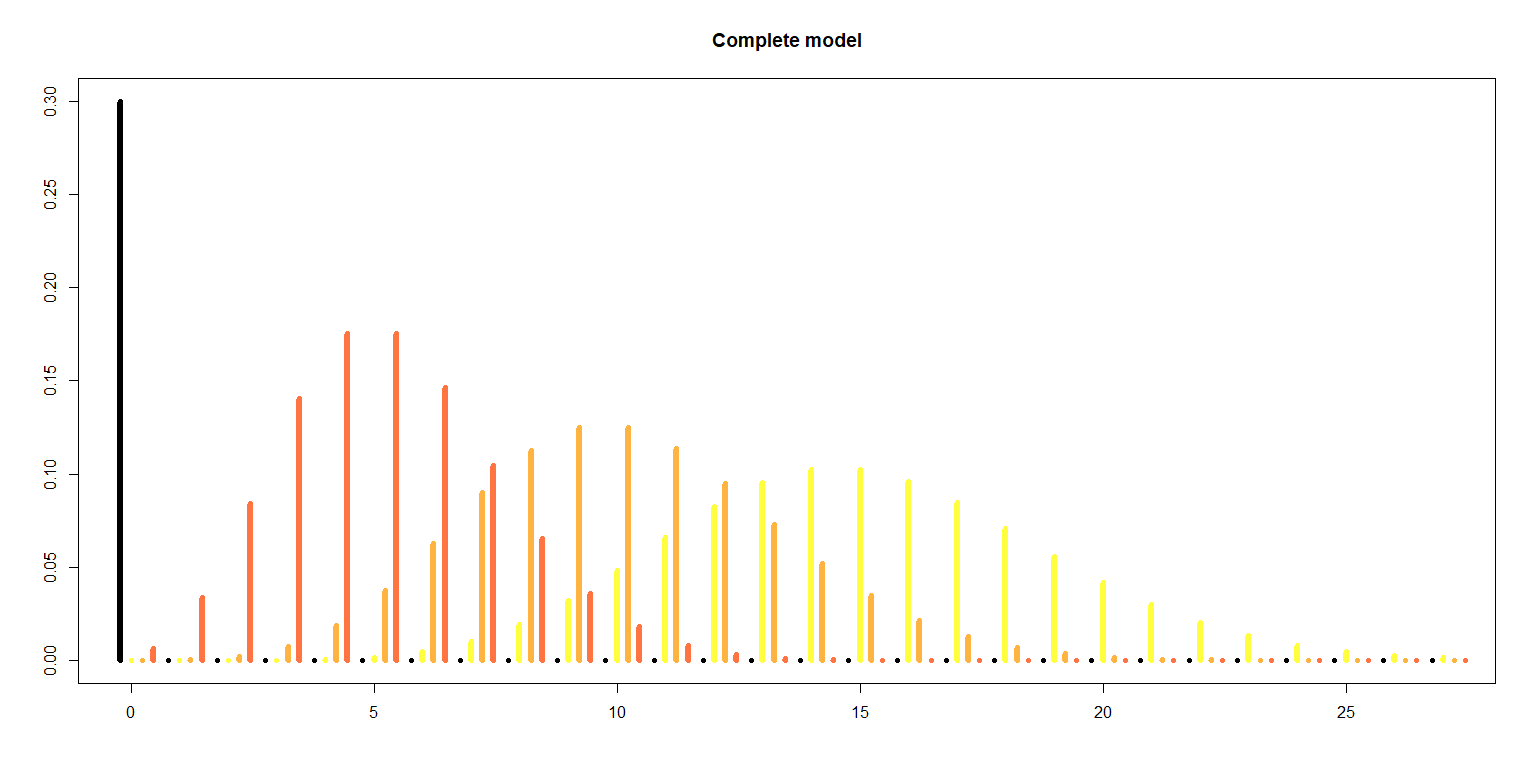
\includegraphics[width=1\linewidth]{pictures/mod3.png} 
	 	\label{fig1}
	 \end{figure}
\end{frame}

\begin{frame}{\textsc{Zero-Inflated Poisson Mixture Regression Model}}

Final model proposed in the paper:

\begin{equation}
\begin{cases}

Y_{ij} \sim \theta \delta_{0} + (1 - \theta)\mathrm{PM}(Y_{ij}|\boldsymbol{\mu}_{ij}, \boldsymbol{\lambda}) \\


\mathrm{PM}(\boldsymbol{\mu}_{ij}, \boldsymbol{\lambda}) = \sum_{k=1}^K \lambda_k\mathrm{Poi}(\mu_{ijk})\\
\mu_{ijk} = \mathrm{exp}\{\boldsymbol{\beta}_k\cdot \mathbf{x}_{ij}\}

\end{cases}
\end{equation}

	where $\theta\in[0,1], \boldsymbol{\lambda} \in Simp(K-1), \, \boldsymbol{\mu}_{ij}\in\mathbb{R}^K,\forall i, j, \  \boldsymbol{\beta}_k\in\mathbb{R}^p,\forall k\in 1\dots K$ are the parameters of the model.\\
	Set priors:
\begin{columns}
\begin{column}{.5\textwidth}
\begin{equation}
\begin{cases}

\boldsymbol{\beta}_k \sim \mathcal{N}(\mathbf{m}_0, \Sigma)\\
\boldsymbol{\lambda} \sim \mathrm{Dirichlet}(\alpha)\\
\theta \sim \mathcal{U}[0,1]

\end{cases}
\end{equation}
\end{column}
\begin{column}{.5\textwidth}
	\alert{Covariates}: strenghts of the adjacent nodes and the geographical distance between the stations.
\end{column}
\end{columns}
	
\end{frame}
\begin{frame}{\textsc{Comments on the Model}}
\begin{columns}[c]
	\hspace{6pt}
	\begin{column}{0.5\textwidth}
		\alert{\textsc{Pros}}\\
		\begin{itemize}
			\item Proper \alert{description of flows}
			\item \alert{interpretable clustering} of the edges inside the network
		\end{itemize}
	\end{column}
	\hspace{5pt}
	\vrule{}
	\hspace{8pt}
	\begin{column}{0.50\textwidth}
		\alert{\textsc{Cons}}\\
		\begin{itemize}
			\item Lack of \alert{day-by-day prediction} of the flow
			\item no distinction between different hours of the day or between various days
		\end{itemize}
	\end{column}
\end{columns}

\end{frame}

\begin{frame}{\textsc{New Challenges}}
\onslide<1,2,3>{
For our project we decided on three main objectives:}
\begin{itemize}
	\onslide<2>{
	\item \alert{\textsc{Autoregressive Model}}
	\\
	Adding the \emph{time dependence} to the model $Y_{ij} \rightarrow Y_{ij}(t)$, with the objective of predicting the network flow for a \alert{new day};
	}
	\onslide<3>{
	\item Introducing \alert{new covariates} to keep track, for instance, of \alert{weekdays} and \alert{weather};
	}
\end{itemize}
\end{frame}

\begin{frame}{\textsc{Impact of Time}}
  WEEKENDS
	\begin{figure}[H]
		\centering
		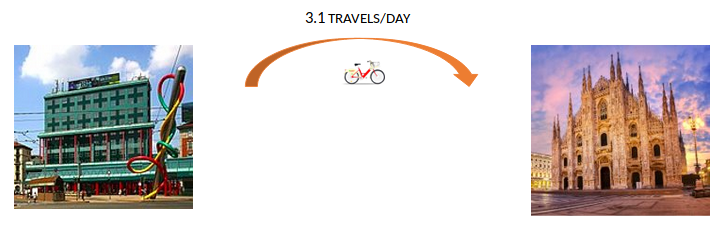
\includegraphics[width=\linewidth]{pictures/WeekEnd.png} 
		\label{fig1}
	\end{figure}
\end{frame}

\begin{frame}{\textsc{Impact of Time}}
WEEKDAYS
\begin{figure}[H]
	\centering
	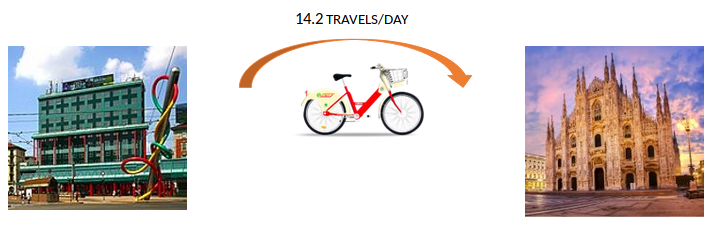
\includegraphics[width=\linewidth]{pictures/WeekDays.png} 
	\label{fig1}
\end{figure}
\end{frame}

\begin{frame}{\textsc{New Challenges}}
For our project we decided on three main objectives:
\begin{itemize}
	\item \alert{\textsc{Autoregressive Model}}
	\\
	Adding the \emph{time dependence} to the model $Y_{ij} \rightarrow Y_{ij}(t)$, with the objective of predicting the network flow for a \alert{new day};
	\item introducing \alert{new covariates} to keep track, for instance, of \alert{weekdays} and \alert{weather};
	\item leaner computations: a \alert{mixed R/C++ implementation}.
\end{itemize}
\end{frame}

\begin{frame}{\textsc{Initial Bibliography}}
 	\begin{itemize}
 		\item \emph{A Bayesian model for network flow data:
 		an application to BikeMi trips};
 		Giulia Bissoli, Celeste Principi, Gian Matteo Rinaldi, Mario Beraha and
 		Alessandra Guglielmi, 2019
 	\end{itemize}
\end{frame}

\end{document}